\documentclass[../notes.tex]{subfiles}

\pagestyle{main}
\renewcommand{\chaptermark}[1]{\markboth{\chaptername\ \thechapter\ (#1)}{}}

\begin{document}




\chapter{Pyridine Chemistry}
\section{Intro, Directed Metallation, and Organometallic Coupling}
\begin{itemize}
    \item \marginnote{1/4:}Announcements.
    \begin{itemize}
        \item This class is a survey course; it is not comprehensive.
        \item This class has a different philosophy from mainstream heterocyclic chemistry; we'll focus not on the "coolest" chemistry, but the chemistry that actually gets used.
        \begin{itemize}
            \item Focus on \emph{Journal of Medicinal Chemistry} and process chem journals.
            \item Steve does not believe that academic research has to be useful, but\dots
            \item Steve believes: Proof is in the pudding. If you're pretending what you're doing has some practical application, you should see it going after 5 years.
        \end{itemize}
        \item Grader: Dr. Dennis Kutateladze.
        \begin{itemize}
            \item He grades the 2 exams; Steve writes both of them.
        \end{itemize}
        \item There are PSets (ungraded, but keys posted).
        \item This is supposed to be a very low-key class; getting a good grade should be easy.
        \begin{itemize}
            \item The goal is to expose you to a lot of different useful chemistry.
            \item Don't look up PSets; goal is not to impress Steve, but to learn the material.
        \end{itemize}
        \item 2 exams + project; (project is graded for completion and effort).
        \begin{itemize}
            \item With 20+ students, probably all of the last 3 classes will be dedicated to presentations.
        \end{itemize}
        \item \textcite{bib:JouleMills} is somewhat dated.
        \begin{itemize}
            \item "A lot of heterocyclic chemistry is ancient."
        \end{itemize}
        \item Organometallic methods come a bit more to the fore in this rendition because Allison isn't currently teaching 5.44 - Organometallic Chemistry.
        \item The final project.
        \begin{itemize}
            \item Most drugs come from the new FDA approvals from last year.
            \item We should put together a 10-minute PowerPoint presentation in which we discuss the disease, how it was discovered, the MedChem synthesis, the process synthesis, the competitors, etc. Emphasis on medchem and process syntheses.
            \item Look at patents, primary papers, etc. Do \emph{not} find a review article and summarize it.
            \item Goal: If we were interested in a compound for our research or job, how would we go about finding material on it?
        \end{itemize}
    \end{itemize}
    \item Mostly looking at aromatic heterocycles, e.g., not piperidines or tetrahydrofurans.
    \begin{figure}[H]
        \centering
        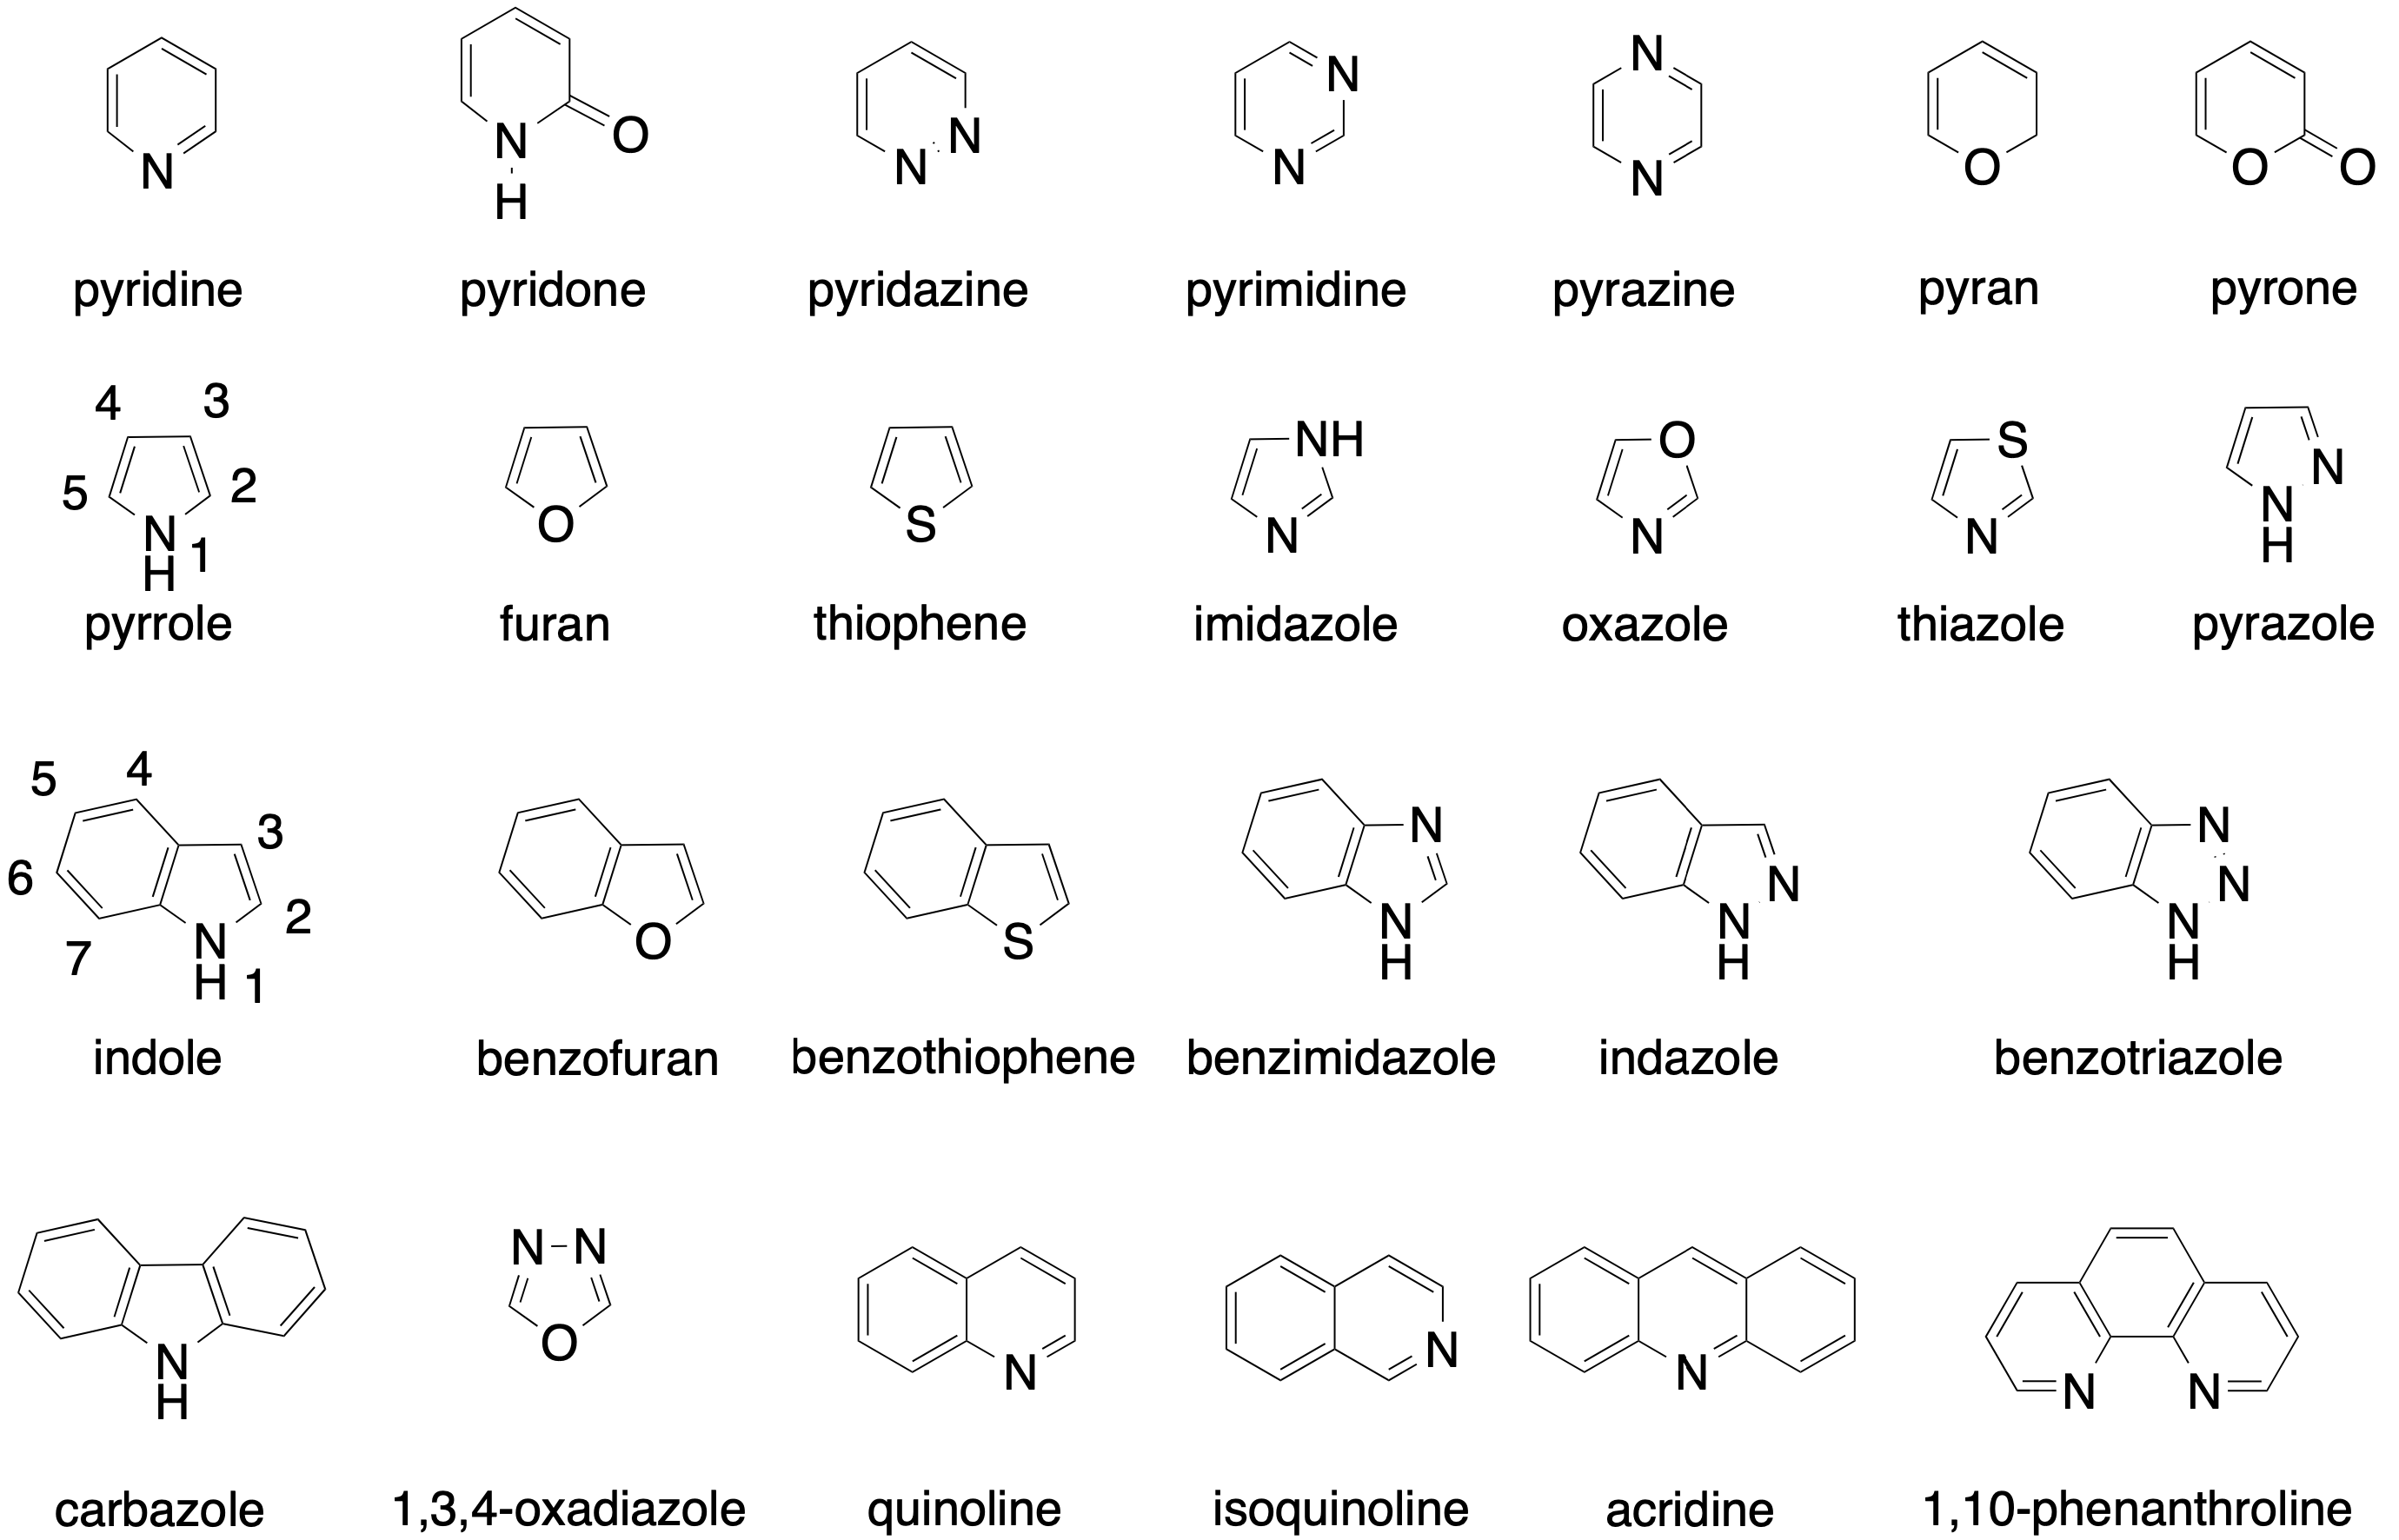
\includegraphics[width=0.8\linewidth]{heterocycles.png}
        \caption{Heterocycles of interest.}
        \label{fig:heterocycles}
    \end{figure}
    \begin{itemize}
        \item We don't need to know the names of all the heterocycles, but we should learn the big ones!!
        \item Interesting heterocycles often contain because it can be protonated, and it hydrogen bonds.
        \begin{itemize}
            \item Hydrogen bonding is useful for receptors, salt bridges, etc.
        \end{itemize}
        \item Salts of these compounds usually imply some kind of water solubility.
        \item \textbf{Pharmacokinetics} are often moderated by heterocycles.
        \begin{itemize}
            \item Making the drug hang around for the right amount of time is super important, because the more times per day people have to take the drugs, the more that compliance goes down (especially among the elderly population).
        \end{itemize}
    \end{itemize}
    \item Blockbuster drugs.
    \begin{itemize}
        \item Several examples given.
        \item Imbruvica Janssen is a covalent drug, doing a Michael addition to DNA.
    \end{itemize}
    \item Infamous drugs.
    \begin{itemize}
        \item Lipitor.
        \begin{itemize}
            \item A \textbf{statin}, i.e., a cholesterol-lowering agent.
            \item One of the most important drugs in the last century in extending people's lifetimes.
            \item Anyone over 50 either has taken one (or should take one, in Steve's opinion!).
        \end{itemize}
        \item Quinine.
        \begin{itemize}
            \item Anti-malarial.
            \item Also in gin and tonics!
        \end{itemize}
        \item Strychnine.
        \begin{itemize}
            \item Rat poison.
            \item Big target in synthetic chemistry, starting with Woodward.
        \end{itemize}
        \item $\beta$-lactam antibiotics.
        \begin{itemize}
            \item Penicillin, and the ring-expanded cephalexins.
        \end{itemize}
        \item Thalidomide.
        \begin{itemize}
            \item Caused the big push for the sale of single-enantiomer drugs!
        \end{itemize}
    \end{itemize}
    \item Pyridine.
    \begin{itemize}
        \item Horrible-smelling, polar solvent.
        \item Originally came from coal tar (precursor to petroleum).
    \end{itemize}
    \item Current synthesis of pyridine.
    \begin{equation*}
        \ce{CH3CHO + H2CO + NH3 ->[vapor phase][Si/Al cat] Py + 3-MePy}
    \end{equation*}
    \begin{itemize}
        \item This synthesis is carried out with flow chemistry.
        \begin{itemize}
            \item Before it was trendy in pharma, it is the only thing that was \emph{ever} used in the production of commodity chemicals.
            \item When you're making commodity chemicals, you can't afford solvents or separations.
        \end{itemize}
        \item It produces pyridine on a scale of 20,000 tons per year.
    \end{itemize}
    \item Aside: Many chemicals are produced from such "magic reactions."
    \begin{itemize}
        \item Example: Acrylonitrile.
        \begin{itemize}
            \item Industrial synthesis: Mix propene and ammonia with a molybdenum/vanadium catalyst.
        \end{itemize}
        \item Example: THF.
        \begin{itemize}
            \item Industrial synthesis: From butane!
        \end{itemize}
        \item "I mean, how?! Write a mechanism for that!"
    \end{itemize}
    \item Many drugs contain pyridine moieties. Here are some examples.
    \begin{itemize}
        \item Muscopyridine: Perfumes.
        \item Prevacid: Acid reflux.
        \item Nexium: Sold as a single-enantiomer with a stereogenic sulfur atom!
    \end{itemize}
    \item The pharmaceutical industry is largely focused on old people because it's a huge market share.
    \begin{itemize}
        \item Pain, sleep, etc. are huge.
        \item As you get older, your body starts to break down.
        \item Alzheimers is a big target, but not much success so far.
    \end{itemize}
    \item The structure of pyridine.
    \begin{figure}[H]
        \centering
        \begin{subfigure}[b]{\linewidth}
            \centering
            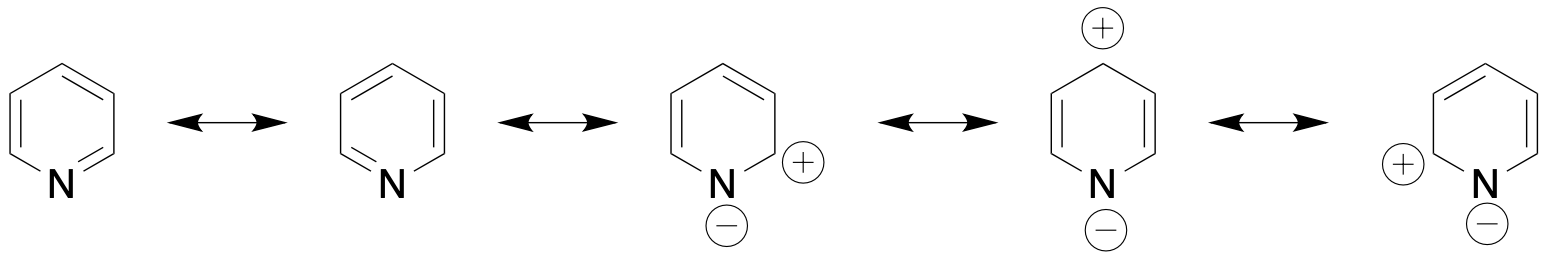
\includegraphics[width=0.7\linewidth]{PyStructurea.png}
            \caption{Important resonance forms.}
            \label{fig:PyStructurea}
        \end{subfigure}\\[1em]
        \begin{subfigure}[b]{0.3\linewidth}
            \centering
            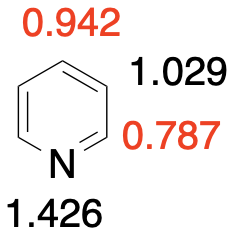
\includegraphics[width=0.39\linewidth]{PyStructureb.png}
            \caption{$\pi$-electron populations.}
            \label{fig:PyStructureb}
        \end{subfigure}
        \begin{subfigure}[b]{0.3\linewidth}
            \centering
            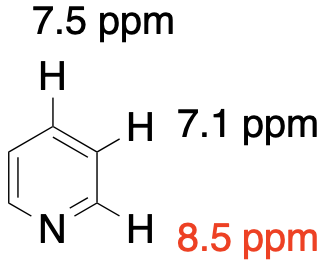
\includegraphics[width=0.55\linewidth]{PyStructurec.png}
            \caption{\ce{{}^1H} NMR shifts.}
            \label{fig:PyStructurec}
        \end{subfigure}
        \caption{Pyridine structure.}
        \label{fig:PyStructure}
    \end{figure}
    \begin{itemize}
        \item Analogous to benzene; slightly less aromatic, but very similar.
        \item Insights from the \ce{{}^1H} NMR.
        \begin{itemize}
            \item \emph{ortho}-proton shifts significantly downfield, \emph{meta}-proton is largely unaffected, and \emph{para}-proton shifts downfield a bit.
            \item This is because there are resonance structures where we put $\delta^+$ on the 2,4,6-positions, while the \emph{meta}-positions take a slight $\delta^-$.
        \end{itemize}
        \item Strong dipole (\SI{2.2}{\debye}) toward the nitrogen atom.
        \item More $\pi$-electron density on nitrogen than anything else.
    \end{itemize}
    \item Reactivity of pyridine.
    \begin{itemize}
        \item Can be reduced to piperidines, sometimes with selectivity, sometimes enantioselectively.
        \item Minisci-type radical reactions.
        \item As an electrophile.
        \item As a Lewis base.
        \item As a Br\o nsted base.
        \item As a nucleophile.
        \item As a reductant.
        \item Very different electrophilic aromatic substitution (EAS) reactivity compared to benzene. You really need activating EDGs with pyridine!
        \item Nucleophilicity is most likely to happen at the nitrogen atom.
        \item S\textsubscript{N}Ar is most likely to happen at the electron-deficient 2,4,6-positions.
        \item EAS is most likely to happen at the relatively electron-rich \emph{meta}-positions.
    \end{itemize}
    \item Pyridine as a base or nucleophile.
    \begin{itemize}
        \item $\pKa\approx 5.5$; much less basic than piperidine.
        \item Basicicity is modulated by EDGs/EWGs.
        \item Pyridine can be transformed from a good to a great nucleophile with some EDGs, e.g., with DMAP.
        \begin{itemize}
            \item DMAP provides rate enhancements of up to $10^4$.
        \end{itemize}
    \end{itemize}
    \item Pyridine reactivity trends.
    \begin{itemize}
        \item Much of pyridine reactivity is driven by\dots
        \begin{itemize}
            \item Avoiding a $\delta^+$ charge on \ce{N}.
            \item That pyridine is a $\pi$-deficient heterocycle (like pyrrole).
        \end{itemize}
        \item Brute force conditions can yield sulfonation.
        \begin{itemize}
            \item The nitrogen would usually react with the electrophile first, and then the product is $10^8$ times less reactive than pyridine, alone.
        \end{itemize}
    \end{itemize}
    \item Nucleophilic aromatic substitution (S\textsubscript{N}Ar) with pyridine.
    \begin{itemize}
        \item Much better with pyridine than with benzene!
        \item Charged intermediates (e.g., where the \ce{N} has coordinated to \ce{E+}) react \emph{exceptionally} fast.
        \item 2,4-chloro is better because you can delocalize the negative charge onto the nitrogen.
    \end{itemize}
    \item Example pyridine reactivity: Biological oxidation of alcohols to aldehydes.
    \begin{itemize}
        \item Done with \ce{NAD+} and a pyridine derivative!
    \end{itemize}
    \item Pyridones.
    \begin{figure}[H]
        \centering
        \footnotesize
        \schemestart
            \chemfig{*6(-N=(-OH)-=-=)}
            \arrow{<->>}
            \chemfig{*6(-\chembelow{N}{H}-(=O)-=-=)}
        \schemestop
        \caption{Pyridone tautomerization.}
        \label{fig:pyridoneTaut}
    \end{figure}
    \begin{itemize}
        \item 2-pyridone (Figure \ref{fig:pyridoneTaut}): Both tautomers are aromatic, but pyridone has stronger BDEs.
        \item 4-pyridone: Still the ketone form.
        \item 3-pyridone: Forms the zwitterion.
    \end{itemize}
    \item Pyridone reactivity.
    \begin{figure}[h!]
        \centering
        \footnotesize
        \begin{subfigure}[b]{\linewidth}
            \centering
            \schemestart
                \chemfig{*6(-\chembelow{N}{H}(-[6,0.4,,,opacity=0])-(=O)-=-=)}
                \arrow{->[\ce{POCl3}][base]}[,1.2]
                \chemfig{*6(-N(-[6,0.4,,,opacity=0])=(-Cl)-=-=)}
            \schemestop
            \caption{The reaction.}
            \label{fig:pyridoneCla}
        \end{subfigure}\\[2em]
        \begin{subfigure}[b]{\linewidth}
            \centering
            \schemestart
                \chemfig{*6(-N(-[@{11}]@{1H}H)-[@{12,0.4}](=[@{13}]O)-=-=)}
                \arrow{->[{\chemfig[atom sep=1.4em]{@{2P}P(=[2]O)(-[@{21}:-30]@{2Cl}Cl)(-[6]Cl)(-[:-150]Cl)}}][\chemfig{@{3B}\charge{180=\:}{B}}]}[,1.6]
                \chemfig{*6(-@{4N}N(-[,,,,opacity=0]\phantom{H})=[@{41}]@{4C}(-O-[:30]POCl_2)-(-[:20,0.5,,,opacity=0]@{4Cl}\charge{[extra sep=4pt]45=$\ominus$}{Cl})=-=)}
                \arrow
                \chemfig{*6(-@{5N}\charge{[extra sep=5pt]-90=$\ominus$}{N}(-[,,,,opacity=0]\phantom{H})-[@{51}](-[@{52}:-50]O-[@{53}:10]POCl_2)(-[:-10]Cl)-=-=)}
                \arrow{->[-\ce{PO2Cl}][-\ce{HCl}]}[,1.3]
                \chemfig{*6(-N(-[6,0.4,,,opacity=0])=(-Cl)-=-=)}
            \schemestop
            \chemmove{
                \draw [curved arrow={6pt}{2pt}] (3B) to[out=180,in=0] (1H);
                \draw [curved arrow={2pt}{2pt}] (11) to[bend right=60,looseness=1.5] (12);
                \draw [curved arrow={3pt}{2pt}] (13) to[out=60,in=150] (2P);
                \draw [curved arrow={2pt}{2pt}] (21) to[bend left=80,looseness=3] (2Cl);
                % 
                \draw [curved arrow={10pt}{2pt}] (4Cl) to[out=45,in=25,out looseness=2,in looseness=4] (4C);
                \draw [curved arrow={4pt}{2pt}] (41) to[bend right=80,looseness=3] (4N);
                % 
                \draw [curved arrow={10pt}{2pt}] (5N) to[out=-90,in=-70,out looseness=4.5,in looseness=4] (51);
                \draw [curved arrow={2pt}{2pt}] (52) to[bend right=100,looseness=2.5] (53);
            }
            \caption{The mechanism.}
            \label{fig:pyridoneClb}
        \end{subfigure}
        \caption{Pyridone chlorination.}
        \label{fig:pyridoneCl}
    \end{figure}
    \begin{itemize}
        \item \ce{POCl3} is one of the most used species in heterocyclic chemistry.
        \item It works so well because \ce{P=O} bond formation is an \emph{excellent} driving force.
    \end{itemize}
    \item Directed metallation --- see \textcite{bib:5-511Notes}.
    \begin{itemize}
        \item Has been around for a while.
        \begin{itemize}
            \item Sigma-Aldrich catalogs have thousands of monosubstituted aromatics, probably still thousands of disubstituted aromatics, but very few (very expensive) tri-substituted aromatics.
            \item Example: Buy anisole, and then you can very easily upgrade it with directed metallation.
        \end{itemize}
        \item Pioneers: Victor Snieckus (Queen's University) and Peter Beak (UIUC).
        \item Two mechanistic theories: Binding to the functional group, and an inductive effect of acidification.
        \begin{itemize}
            \item An expert in lithium chemistry at Cornell has shown that the inductive effect is more important, at least in the case of anisole, contrary to 5.511!
        \end{itemize}
        \item Per Steve, this is one of the most important transformations in organic chemistry.
        \item Common directing groups.
        \begin{itemize}
            \item Aryl ethers, $3^\circ$ amides, MOM ethers, $3^\circ$ carbamates, and $3^\circ$ sulfonamides.
            \item For $\pi$-deficient heterocycles (e.g., pyridine), also: \ce{F}, \ce{Cl}, \ce{Br}, \ce{CF3}, \ce{CO2-}.
        \end{itemize}
        \item References: \textcite{bib:DMGRev1}, \textcite{bib:DMGRev2}, \textcite{bib:DMGRev3}.
    \end{itemize}
    \pagebreak
    \item Pyridine preferably undergoes metallation \emph{not} adjacent to the nitrogen.
    \begin{itemize}
        \item \ce{N-Li} binding kinetically favors lithiation at the \emph{ortho}-positions.
        \item However, having two lone pairs so close together is thermodynamically disfavored, presumably because of Coulombic repulsion between the electron pairs, i.e., the \textbf{$\bm{\alpha}$-effect}.
        \item Indeed, lithiation actually prefers to happen at the more acidic \emph{para}-position, which is still $\delta^+$ but has less coulombic repulsion.
        \item Remember that $\pKa$ is a \emph{thermodynamic} function.
    \end{itemize}
    \item DMGs on pyridine.
    \begin{itemize}
        \item Most \emph{meta}-DMGs direct to the \emph{para}-position: \ce{Cl}, \ce{F}, MOM ethers, siloxane ethers, bulky $3^\circ$ amides (e.g., \ce{C(O)N{}^{\emph{i}}Pr2}), and bulky amides bonded through the nitrogen.
        \item \emph{meta}-\ce{OEt} directs to the \emph{ortho}-position.
        \item Review some typical lithiation and functionalization reactions from 5.511.
        \begin{itemize}
            \item LDA lithiates 3-chloropyridine at $-\SI{23}{\celsius}$ instead of eliminating to the benzyne derivative (as it would at a higher temperature).
        \end{itemize}
        \item References lithium halogen exchange.
    \end{itemize}
    \item Lateral deprotonations.
    \begin{itemize}
        \item \emph{ortho}- and \emph{para}-methylpyridine like to deprotonate "benzylically" much more than toluene because of additional nitrogen stabilization.
        \begin{itemize}
            \item Indeed, the $\pKa$ of the 2,3,4-positions is 29.5, 33.5, and 26, respectively.
            \item In contrast, toluene's $\pKa$ is 42.
        \end{itemize}
        \item Decarboxylation can be useful for substitution reactions.
        \begin{itemize}
            \item Example: Mixing 2-pyridylacetic acid with a base leads to decarboxylation and the formation of 2-methylpyridine upon workup.
        \end{itemize}
        \item Thermodynamic vs. kinetic lateral deprotonations.
        \begin{itemize}
            \item Consider 2,4-dimethylpyridine.
            \item Bases of comparable strength (e.g., LDA) deprotonate thermodynamically at the 4-position.
            \item Stronger bases with aggregates broken up by the directing nitrogen (e.g., \ce{{}^{\emph{n}}BuLi}) deprotonate kinetically at the 2-position.
            \item Interestingly, adding \ce{{}^{\emph{n}}BuLi} and then an amine base allows for equilibration from the kinetic 2-lithiated to the thermodynamic 4-lithiated species!
            \item Reference: \textcite[90]{bib:PyLatThermKin}.
        \end{itemize}
    \end{itemize}
    \item How could we convert 2-chloro to 2-methylpyridine?
    \begin{figure}[h!]
        \centering
        \vspace{-2em}
        \footnotesize
        \schemestart
            \chemfig{*6(-N=(-Cl)-=-=)}
            \arrow{0}[,0.1]\+{,,-2pt}
            \chemfig{\charge{[extra sep=5pt]180=$\ominus$}{}(-[:60]CO_2Me)(-[:-60]CO_2Me)-[4,0.5,,,opacity=0]}
            \arrow
            \chemfig{*6(-N=(-(-[:30]CO_2Me)(-[6]CO_2Me))-(-[,,,,opacity=0]-[2,,,,opacity=0]\phantom{CO_2Me})=-=)}
            \arrow{->[\ce{HO-}][$\Delta$]}
            \chemfig{*6(-N=(-Me)-=-=)}
        \schemestop
        \caption{Lateral pyridine decarboxylation in robust synthesis.}
        \label{fig:PyLatCO2}
    \end{figure}
    \begin{itemize}
        \item General rule: If you can use chemistry from the 1920s, it will work better than chemistry from the 2020s.
        \item Lab scale: Do cross-coupling with methyl boronic acid and a palladium catalyst.
        \item 100 ton scale: Use a malonate anion and then double decarboxylation.
    \end{itemize}
    \item Pyridines as ylide-like species.
    \begin{figure}[H]
        \centering
        \begin{subfigure}[b]{\linewidth}
            \centering
            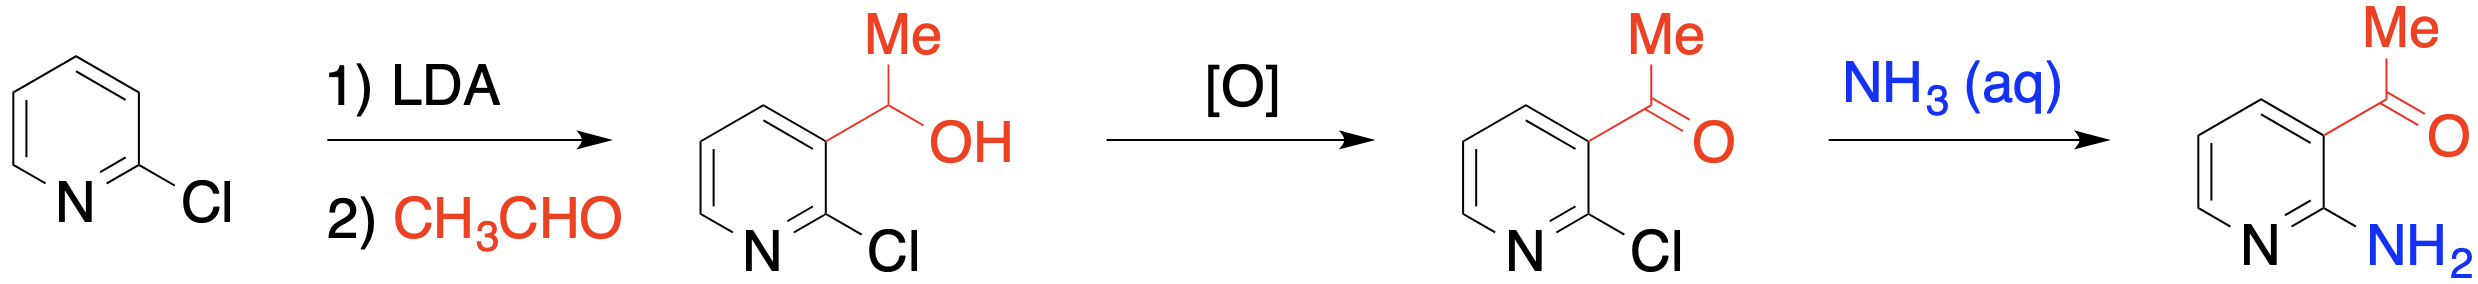
\includegraphics[width=0.85\linewidth]{PyMultifunca.png}
            \caption{Preparation of pyridyne "ylides."}
            \label{fig:PyMultifunca}
        \end{subfigure}\\[2em]
        \begin{subfigure}[b]{\linewidth}
            \centering
            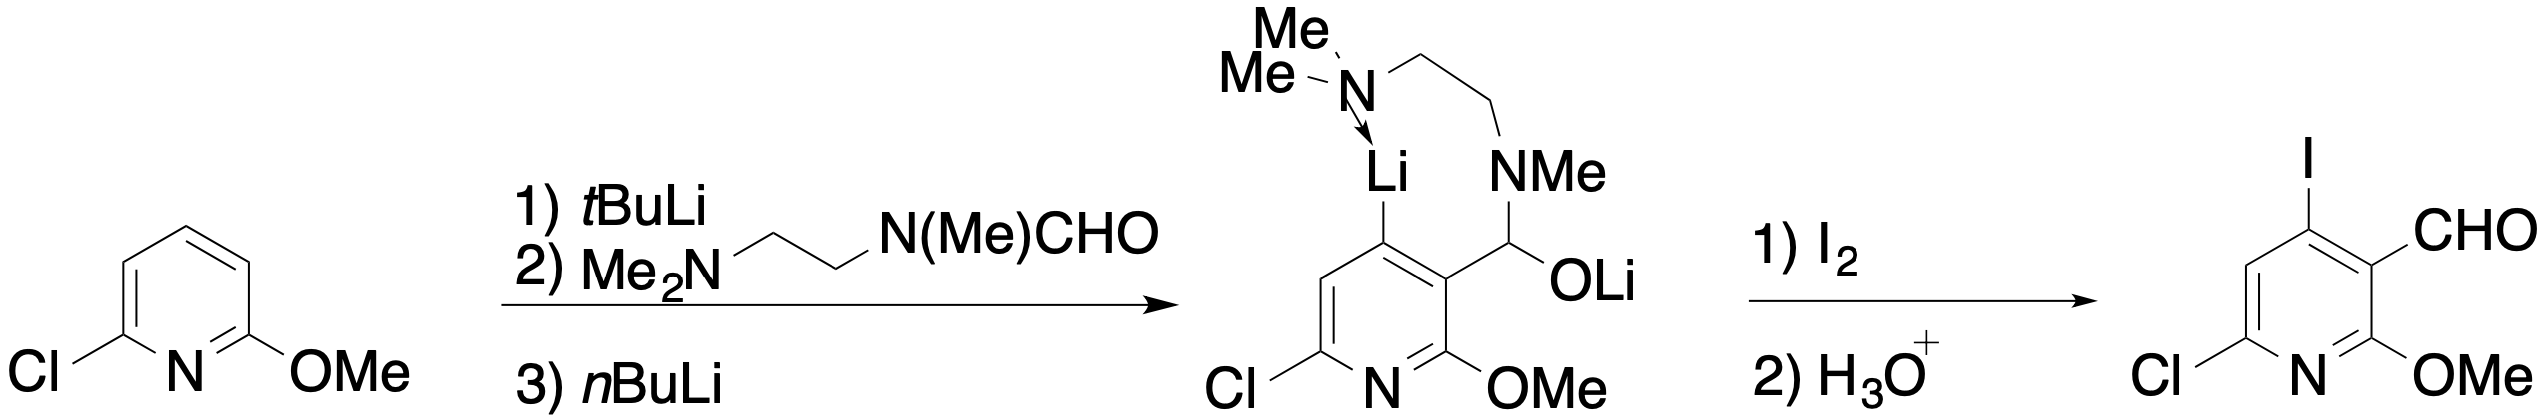
\includegraphics[width=0.85\linewidth]{PyMultifuncb.png}
            \caption{3,4-difunctionalization.}
            \label{fig:PyMultifuncb}
        \end{subfigure}
        \caption{Multifunctionalization of pyridines.}
        \label{fig:PyMultifunc}
    \end{figure}
    \begin{itemize}
        \item You can form what is essentially a ylide between the 2- and 3-positions of the pyridyne by adding an EWG adjacent to a S\textsubscript{N}Ar position (Figure \ref{fig:PyMultifunca}).
        \begin{itemize}
            \item Essentially, we begin with a species that has a DMG which can also (later on) do S\textsubscript{N}Ar.
            \item We use it as a DMG to functionalize the adjacent position with an EWG of interest.
            \item The EWG makes the ring even more activated toward S\textsubscript{N}Ar.
            \item Thus, we've essentially added a nucleophile and electrophile to pyridine very quickly.
        \end{itemize}
        \item Can get fancier with 3,4-disubstitutions (Figure \ref{fig:PyMultifuncb}).
        \begin{itemize}
            \item The stronger methoxy DMG lithiates at the 3-position. We then add a TMEDA-like species and use it to lithiate at the 4-position.
            \item An electrophile can then add at the 4-position, and we can cleave off TMEDA with an acid workup.
        \end{itemize}
        \item Steve skips the last reaction (using a \emph{para}-carbamate to asymetrically functionalize both \emph{meta}-positions).
    \end{itemize}
    \item Aside on medchem.
    \begin{itemize}
        \item \emph{Yield} and \emph{ee} are things we fixate on as academics, but medicinal chemists don't care.
        \item "People who are unsuccessful spend a lot of time optimizing something that doesn't end up working out."
        \item It's much more important to be able to get a mockup of the drug to test, and then they'll get a better working reaction later if need be.
    \end{itemize}
    \item The \textbf{Chichibabin reaction}.
    \begin{figure}[h!]
        \centering
        \footnotesize
        \schemestart
            \chemfig{*6(-N=-=-=)}
            \arrow{->[\ce{NaNH2}][\SI{160}{\celsius}, Tol]}[,1.6]
            \chemfig{*6(-N=(-NH_2)-=-=)}
        \schemestop
        \caption{Chichibabin reaction.}
        \label{fig:chichibabin}
    \end{figure}
    \begin{itemize}
        \item Makes 2-aminopyridine from pyridine.
    \end{itemize}
    \pagebreak
    \item Activating pyridine toward $sp^2$- and $sp$-Grignard reagents.
    \begin{itemize}
        \item If we treat pyridine with an acid chloride or other EWG, it adds in to form an activated `amide.'
        \item We can then easily do S\textsubscript{N}Ar at the 2-position with \ce{ArMgX}, \ce{ViMgX}, or an alkynyl Grignard.
        \item This reaction is \emph{not} selective for alkyl Grignards.
    \end{itemize}
    \item Pyridine isn't very good at EAS, but pyridine \emph{N}-oxide can do it better.
    \item Synthesis of a pyridine \emph{N}-oxide.
    \begin{figure}[h!]
        \centering
        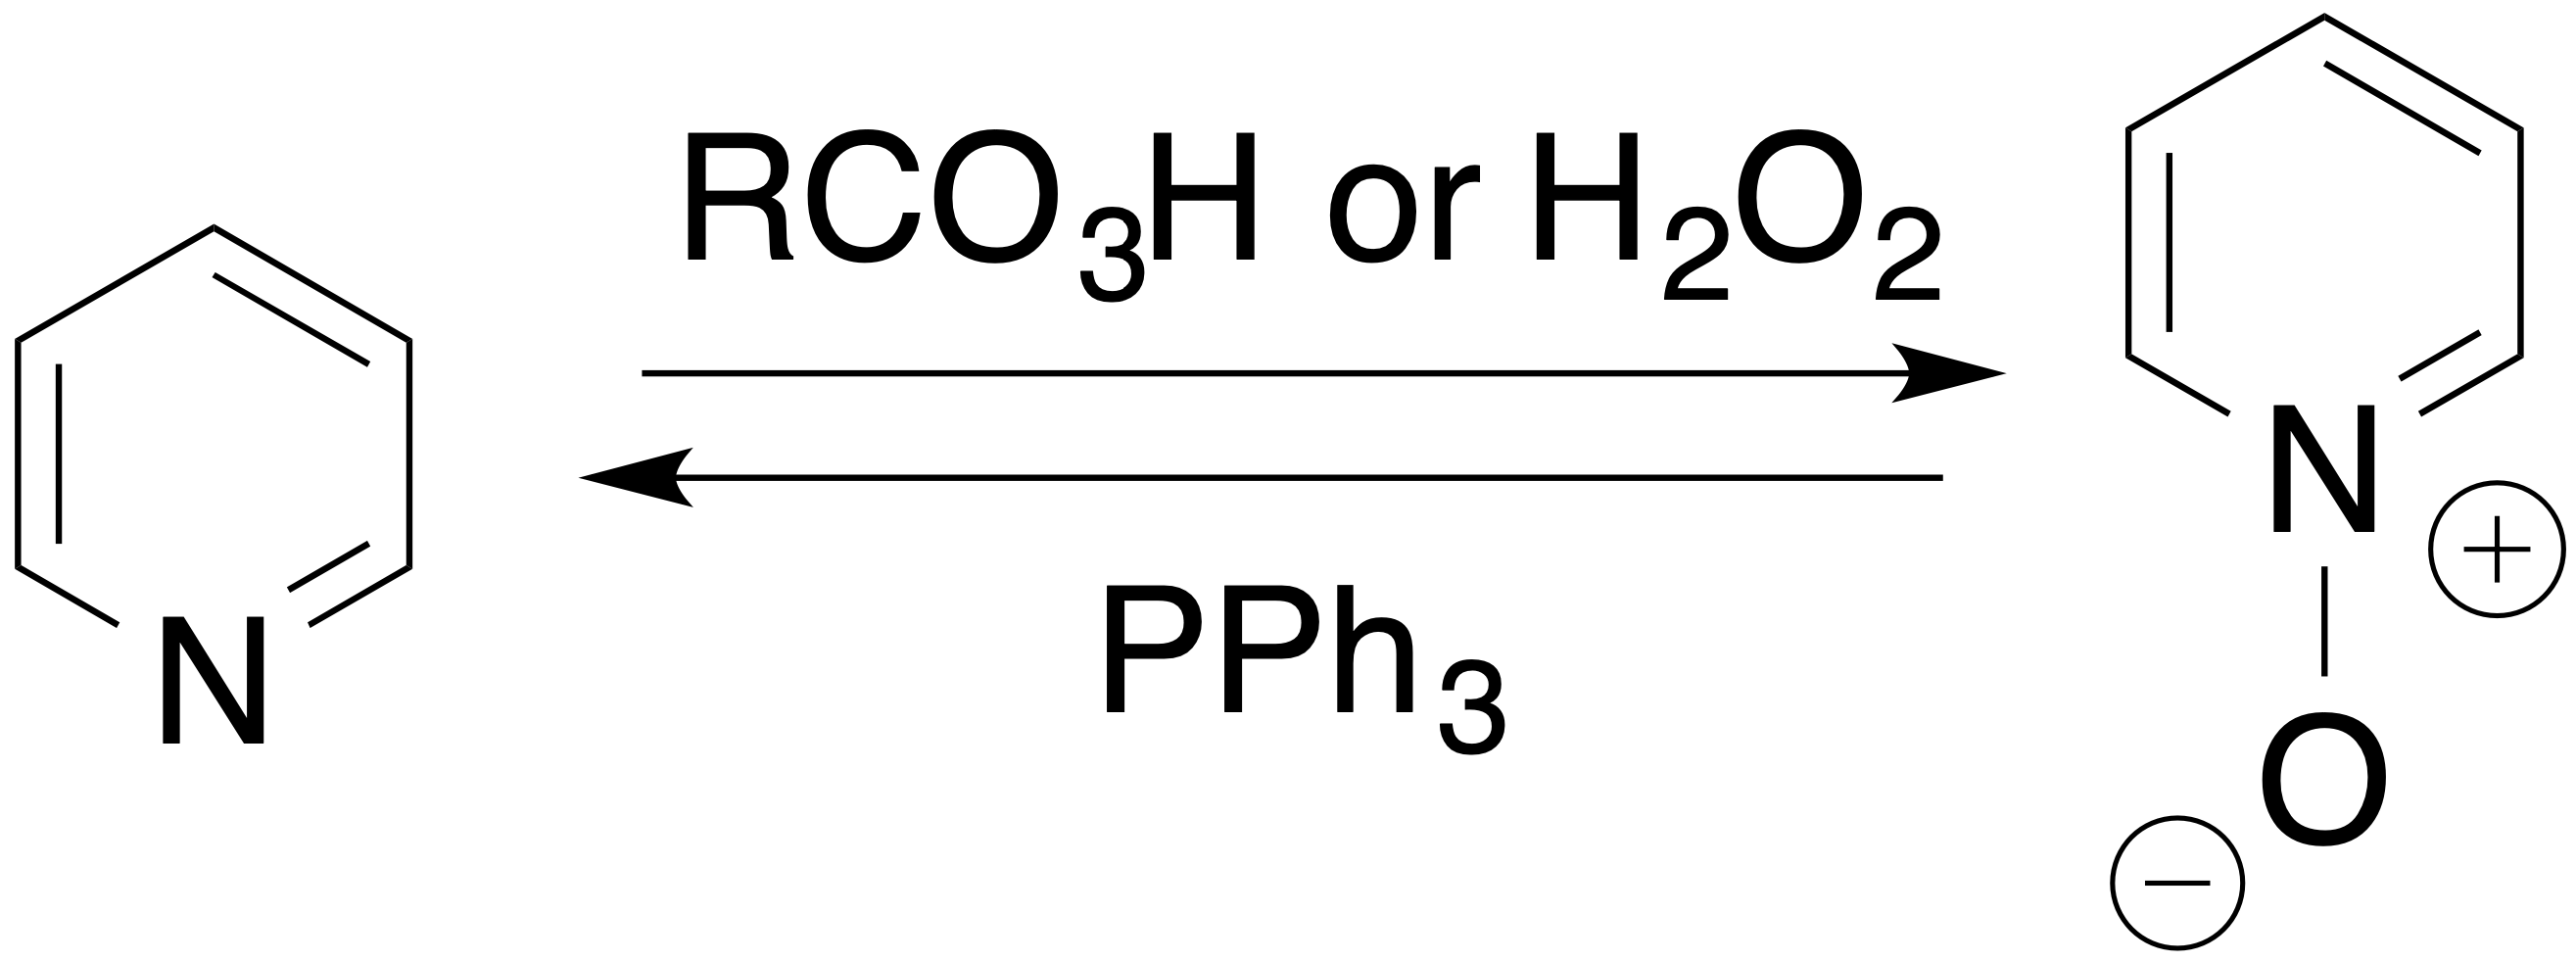
\includegraphics[width=0.3\linewidth]{PyNO.png}
        \caption{Synthesis of pyridine \emph{N}-oxides.}
        \label{fig:PyNO}
    \end{figure}
    \begin{itemize}
        \item Reversibly synthesize with peroxides, and \ce{PPh3}.
    \end{itemize}
    \item The counterintuitive result of pyridine oxidation is that the ring becomes \emph{more} electron-rich, because now the oxyanion's lone pairs donate in!
    \begin{itemize}
        \item Thus, for example, pyridine \emph{N}-oxide reacts under nitration conditions to yield 4-nitropyridine \emph{N}-oxide.
        \item As another example, \textbf{fuming sulfuric acid} and bromine lead to bromination at the 3-position.
        \begin{itemize}
            \item This is because the reaction is thought to proceed via oxygen coordination to \ce{HSO3+}.
        \end{itemize}
        \item \ce{POCl3} can also covert pyridine \emph{N}-oxide to 2-chloropyridine.
        \begin{itemize}
            \item BMS and Phil Baran have somewhat supplanted this reaction \parencite{bib:PyNOCl}.
        \end{itemize}
    \end{itemize}
    \item \textbf{Fuming sulfuric acid}: A mixture of \ce{H2SO4} and \ce{SO3}.
    \item We now move onto transition metal-catalyzed cross-coupling.
    \item TM-catalyzed cross-coupling has revolutionized the pharmaceutical industry, and somewhat distorted it.
    \begin{itemize}
        \item New drugs have a lot of biaryls because they're easy to make, probably not because they're optimal.
        \item Few reactions work with as much generality and substrate scope as cross-coupling.
    \end{itemize}
    \item Steve reviews the typical catalytic cycle for cross-coupling.
    \item Top reactions in the pharmaceutical industry.
    \begin{itemize}
        \item Amide-bond formation (huge!), and reductive amination.
    \end{itemize}
    \item List of cross-coupling reactions.
    \begin{itemize}
        \item Usually palladium- or nickel-catalyzed; some with copper.
        \item Kumada and Corriu developed a nickel-catalyzed cross-coupling that would have won the Nobel prize except that Kumada died.
        \item Negishi realized that a lot of magnesium reagents had functional group compatability issues.
        \begin{itemize}
            \item He went through zirconium before he got to zinc.
        \end{itemize}
        \item Stille probably had the best coupling, but he died in a plane crash. Functional group compatability and ease of separation of products is ideal with this, but it's not used as much any more due to toxicity concerns.
        \item Miyaura was an associate professor under Suzuki at Hokkaido who actually discovered this stuff.
        \begin{itemize}
            \item Most widely used because of ease and low toxicity.
        \end{itemize}
        \item Heck probably understood the chemistry the best; he was a remarkable individual in Steve's estimation.
        \begin{itemize}
            \item 7 single author back-to-back ($\times 7$) JACS publications.
            \begin{itemize}
                \item References: \textcite{bib:Heck1}, \textcite{bib:Heck2}, \textcite{bib:Heck3}, \textcite{bib:Heck4}, \textcite{bib:Heck5}, \textcite{bib:Heck6}, and \textcite{bib:Heck7}.
            \end{itemize}
            \item Timing is everything, and he published it too early.
            \item He was retired by the time he won the Nobel prize.
        \end{itemize}
        \item Ullmann was one of the first.
        \item Carbonylation: Aryl palladium with CO forms the acyl palladium that reacts just like an acid halide.
    \end{itemize}
    \item Ligands for CC.
    \begin{itemize}
        \item \ce{Pd(PPh3)4} is classic.
        \item Large bulky things turn out to be better.
        \item Having a bottom second ring (as in Buchwald ligands) also turns out to be useful.
        \item The principal: \ce{L4Pd} is unreactive; \ce{L2Pd} is quite good but hard to get to; \ce{L1Pd} is ideal. What the different ligands do is change the stability of the coordination environments. Buchwald ligands allow you to get down to \ce{L1Pd} species.
        \item Cone angle and percent buried volume are what is modulated by diarylbialkylphosphines.
        \item Trialkylphosphines and \emph{N}-heterocyclic carbenes can also be useful.
        \item References.
        \begin{itemize}
            \item \textcite{bib:BuchwaldRep} --- Steve's original report of SPhos and XPhos for Suzuki-Miyaura coupling.
            \item \textcite{bib:BuchwaldRev} --- Review of Steve's dialkylphosphinobiaryl ligands.
        \end{itemize}
    \end{itemize}
    \item Suzuki-Miyaura couplings.
    \begin{itemize}
        \item Hundreds of thousands of examples in the literature.
        \item Pd/C leaches a bit and can do the chemistry.
        \item You can also use ligands for more complicated stuff.
    \end{itemize}
\end{itemize}



\section{Pyridine Cross-Coupling, Synthesis, and Derivatization}
\begin{itemize}
    \item \marginnote{2/6:}Announcements.
    \begin{itemize}
        \item I am assigned compound No. 10 for the final project.
        \item PSet 1 posted.
        \begin{itemize}
            \item If you get stuck on a problem, don't do it!
            \item Don't spend more than 3 hours on the PSet.
            \item Spending 27 hours on this PSet demonstrates "a \emph{decided} lack of judgment."
        \end{itemize}
    \end{itemize}
    \item Lecture begins: Back to cross-coupling.
    \pagebreak
    \item A major disadvantage of cross-coupling in synthesis: The amount of catalyst left behind.
    \begin{itemize}
        \item Examples.
        \begin{itemize}
            \item Pd, Rh, Ir: You can have \SI{10}{\partspermillion} residual in your \textbf{API}.
            \item \ce{Ni}: \SI{20}{\partspermillion}.
            \item \ce{Cu}: \SI{300}{\partspermillion}.
        \end{itemize}
        \item API: Active Pharmaceutical Ingredient.
        \item There is a cottage industry of removing trace metals after reaction. Common methods include\dots
        \begin{itemize}
            \item Adsorption onto surfaces;
            \item Oxidation with swimming pool bleach;
            \item Fancier solid-supported resins with ligands.
        \end{itemize}
    \end{itemize}
    \item We'll talk mostly about palladium-catalyzed cross-coupling.
    \begin{itemize}
        \item \ce{Pd} is used in 95\% of applications.
        \begin{itemize}
            \item \ce{Ni} is the other 5\%, since it has decided process benefits (cheaper, lower toxicity).
        \end{itemize}
        \item We add to solution a \textbf{precatalyst} (usually either \ce{Pd^0} or \ce{Pd^{II}}).
        \begin{itemize}
            \item If \ce{Pd^{II}}, you need a reduction.
            \item Contrary to some textbooks, phosphines \emph{cannot} reduce \ce{Pd^{II}}; phosphines \emph{plus water} can.
        \end{itemize}
        \item After reduction (if needed), the precatalyst needs to lose a ligand or two.
        \item $d^8$ metals follow a 16-electron rule, not an 18-electron one.
        \item After oxidative addition to the \emph{cis}-species, you get equilibration to the \emph{trans}-species.
        \item Rate of \emph{oxidative addition} (not the overall catalytic cycle):
        \begin{equation*}
            \ce{I} > \ce{CF3SO3} \approx \ce{Br} \gg \ce{Cl} > \ce{OTs} > \ce{OMs}
        \end{equation*}
        \begin{itemize}
            \item Cost runs in the opposite direction!
            \item If you use a weak catalyst like palladium tetrakis, oxidative addition is rate-limiting. But with active, modern catalysts, ??oxidative addition to?? iodides can be rate limiting!
            \begin{itemize}
                \item Is oxidative addition to iodides slower with modern catalysts, or is it transmetallation with iodides that makes the overall process slower??
            \end{itemize}
        \end{itemize}
        \item Greg Fu (first at MIT, then at Caltech) really pioneered oxidative addition to $sp^3$-halides.
        \begin{itemize}
            \item These substrates did not work previously due to competitive $\beta$-hydride elimination.
            \item Reference: \textcite{bib:FuAlkyl}.
        \end{itemize}
    \end{itemize}
    \item Transmetallation.
    \begin{itemize}
        \item Transfer a group from boron, zinc, tin, etc.
        \item Mechanism: $\sigma$-bond metathesis.
        \begin{itemize}
            \item Note that "metathesis" has nothing to do with olefins; it just means "interchange."
        \end{itemize}
        \item Having an \ce{L1Pd} species means that you have lots of space for $\sigma$-bond metathesis to occur!
        \begin{itemize}
            \item Bulky iodides take up space and can slow this down (with modern catalysts).
            \item Steve has gathered experimental evidence for this effect! See Footnote 18 in \textcite{bib:BuchwaldTransmetal}.
        \end{itemize}
    \end{itemize}
    \item Fu solves heteroaryl boronic acids.
    \begin{equation*}
        \ce{Het1B(OH)2 + Het2X ->[Pd2(dba)3 (1.0 mol\%), PCy3 (2.4 mol\%), K3PO4 (1.7 {eq.})][1,4-dioxane, H2O, \SI{100}{\celsius}] Het1-Het2}
    \end{equation*}
    \begin{itemize}
        \item Very small differences have big impacts on reactivities.
        \item Look at what has been done and don't make assumptions, otherwise you can reinvent problems that have already been solved!
        \item They used \ce{Pd2(dba)2} (dibenzylideneacetone).
        \begin{itemize}
            \item Good, cheap ligand.
            \item Because it's good, it doesn't just say, "goodbye" in the flask; it hangs around and can slow reactivity.
        \end{itemize}
        \item \ce{KF} isn't extremely basic, but boron is very fluorophilic; the ate complex formed facilitates transmetallation.
        \item This is really good heterocycle-heterocycle chemistry!
        \item People have a love-hate relationship with boronic acids.
        \begin{itemize}
            \item Often work but unstable, difficult to quantitate via NMR, etc.
            \item This is why people like to use boronate esters or Molander salts (trifluoroborates), which are both \emph{in situ} slow generators of boronic acids.
            \item Proto-deboronation (replacement of boron with a hydrogen) is a problem, though.
        \end{itemize}
        \item Reference: \textcite{bib:FuHeteroaryls}.
    \end{itemize}
    \item Clever tricks with boron.
    \begin{figure}[h!]
        \centering
        \footnotesize
        \schemestart
            \chemname{
                \chemfig{*6(-=-(-B?-[:15,0.6]O-[:50,0.9](=[:-12]O)-[:110]-[:-170]MeN?[,,{latex-}]-[:-30]-[:-70,,,,ovbnd](=[:-12]O)-[:-130,0.9]O?)=N-=)}
            }{1.5 eq.}
            \arrow{0}[,0.1]\+
            \chemfig{ArCl}
            \arrow{->[\tikz{\node[align=center]{\ce{Pd2(dba)3} (1.5 mol\%)\\XPhos (6 mol\%)\\\ce{Cu(OAc)} (50 mol\%)}}][\tikz{\node[align=center]{\ce{K2CO3}, DMF/IPA\\\SI{100}{\celsius}, 4h}}]}[,2.5]
            \chemfig{*6(-=-(-Ar)=N-=)}
        \schemestop
        \caption{MIDA boronates for air-stable 2-pyridyl couplings.}
        \label{fig:MIDA}
    \end{figure}
    \begin{itemize}
        \item Marty Burke's (UIUC) slow-release strategy generates boronic acid \emph{in situ} as needed.
        \begin{itemize}
            \item Transfer of pyridyl group to copper and then transmetallation.
        \end{itemize}
        \item 2-pyridylboronic acid is extremely unstable; you can buy it, but what you buy won't be it in Steve's opinion.
        \begin{itemize}
            \item Steve believes you should \emph{always} assay your starting materials.
        \end{itemize}
        \item References.
        \begin{itemize}
            \item \textcite{bib:Burke1} --- original report of MIDA boronates.
            \item \textcite{bib:Burke2} --- improved method with copper aminodiol additives.
        \end{itemize}
    \end{itemize}
    \item Negishi coupling of 2-pyridylzinc reagents is ideal!
    \begin{figure}[h!]
        \centering
        \footnotesize
        \setchemfig{autoreset cntcycle=false,fixed length=false}
        \schemestart
            \chemfig{*6(-N=(-ZnBr)-=-=-)}
            \arrow{0}[,0.1]\+
            \chemfig{ArX}
            \arrow{->[\ce{Pd(PPh3)4 (1 mol\%)}][THF, \SI{25}{\celsius}, \SIrange{24}{72}{\hour}]}[,2.4]
            \chemfig{*6((-[,,,,opacity=0])-N=(-Ar)-=-=)}
        \schemestop
        \chemmove{
            \draw [-,ovbnd] (cyclecenter2) ++(-0.2,0) -- ++(-0.45,0) node[left,black]{R};
            \draw [-,ovbnd] (cyclecenter3) ++(-0.2,0) -- ++(-0.45,0) node[left,black]{R};
        }
        \caption{Negishi-type 2-pyridyl couplings.}
        \label{fig:NegishiPyridyl}
    \end{figure}
    \begin{itemize}
        \item No protozincation unless you add water.
        \item Even with the simplest of catalysts, this works.
        \item But much fewer aryl zincs are commercially available.
        \item References: Rieke zinc, \textcite{bib:BuchwaldNegishi} --- RuPhos optimizes Negishi.
    \end{itemize}
    \item Steve's mantra in consulting: The best metal is none.
    \begin{itemize}
        \item If you can do it without a metal, that's ideal.
        \item If you're gonna use a metal, it had better confer a \emph{major} advantage.
        \item Metal catalysis might work on a discovery scale, but uncatalyzed heat will be preferred on a preparative scale.
    \end{itemize}
    \item Dan Weix (Rochester $\to$ Wisconsin-Madison) has pioneered the area of combination catalysts.
    \begin{figure}[h!]
        \centering
        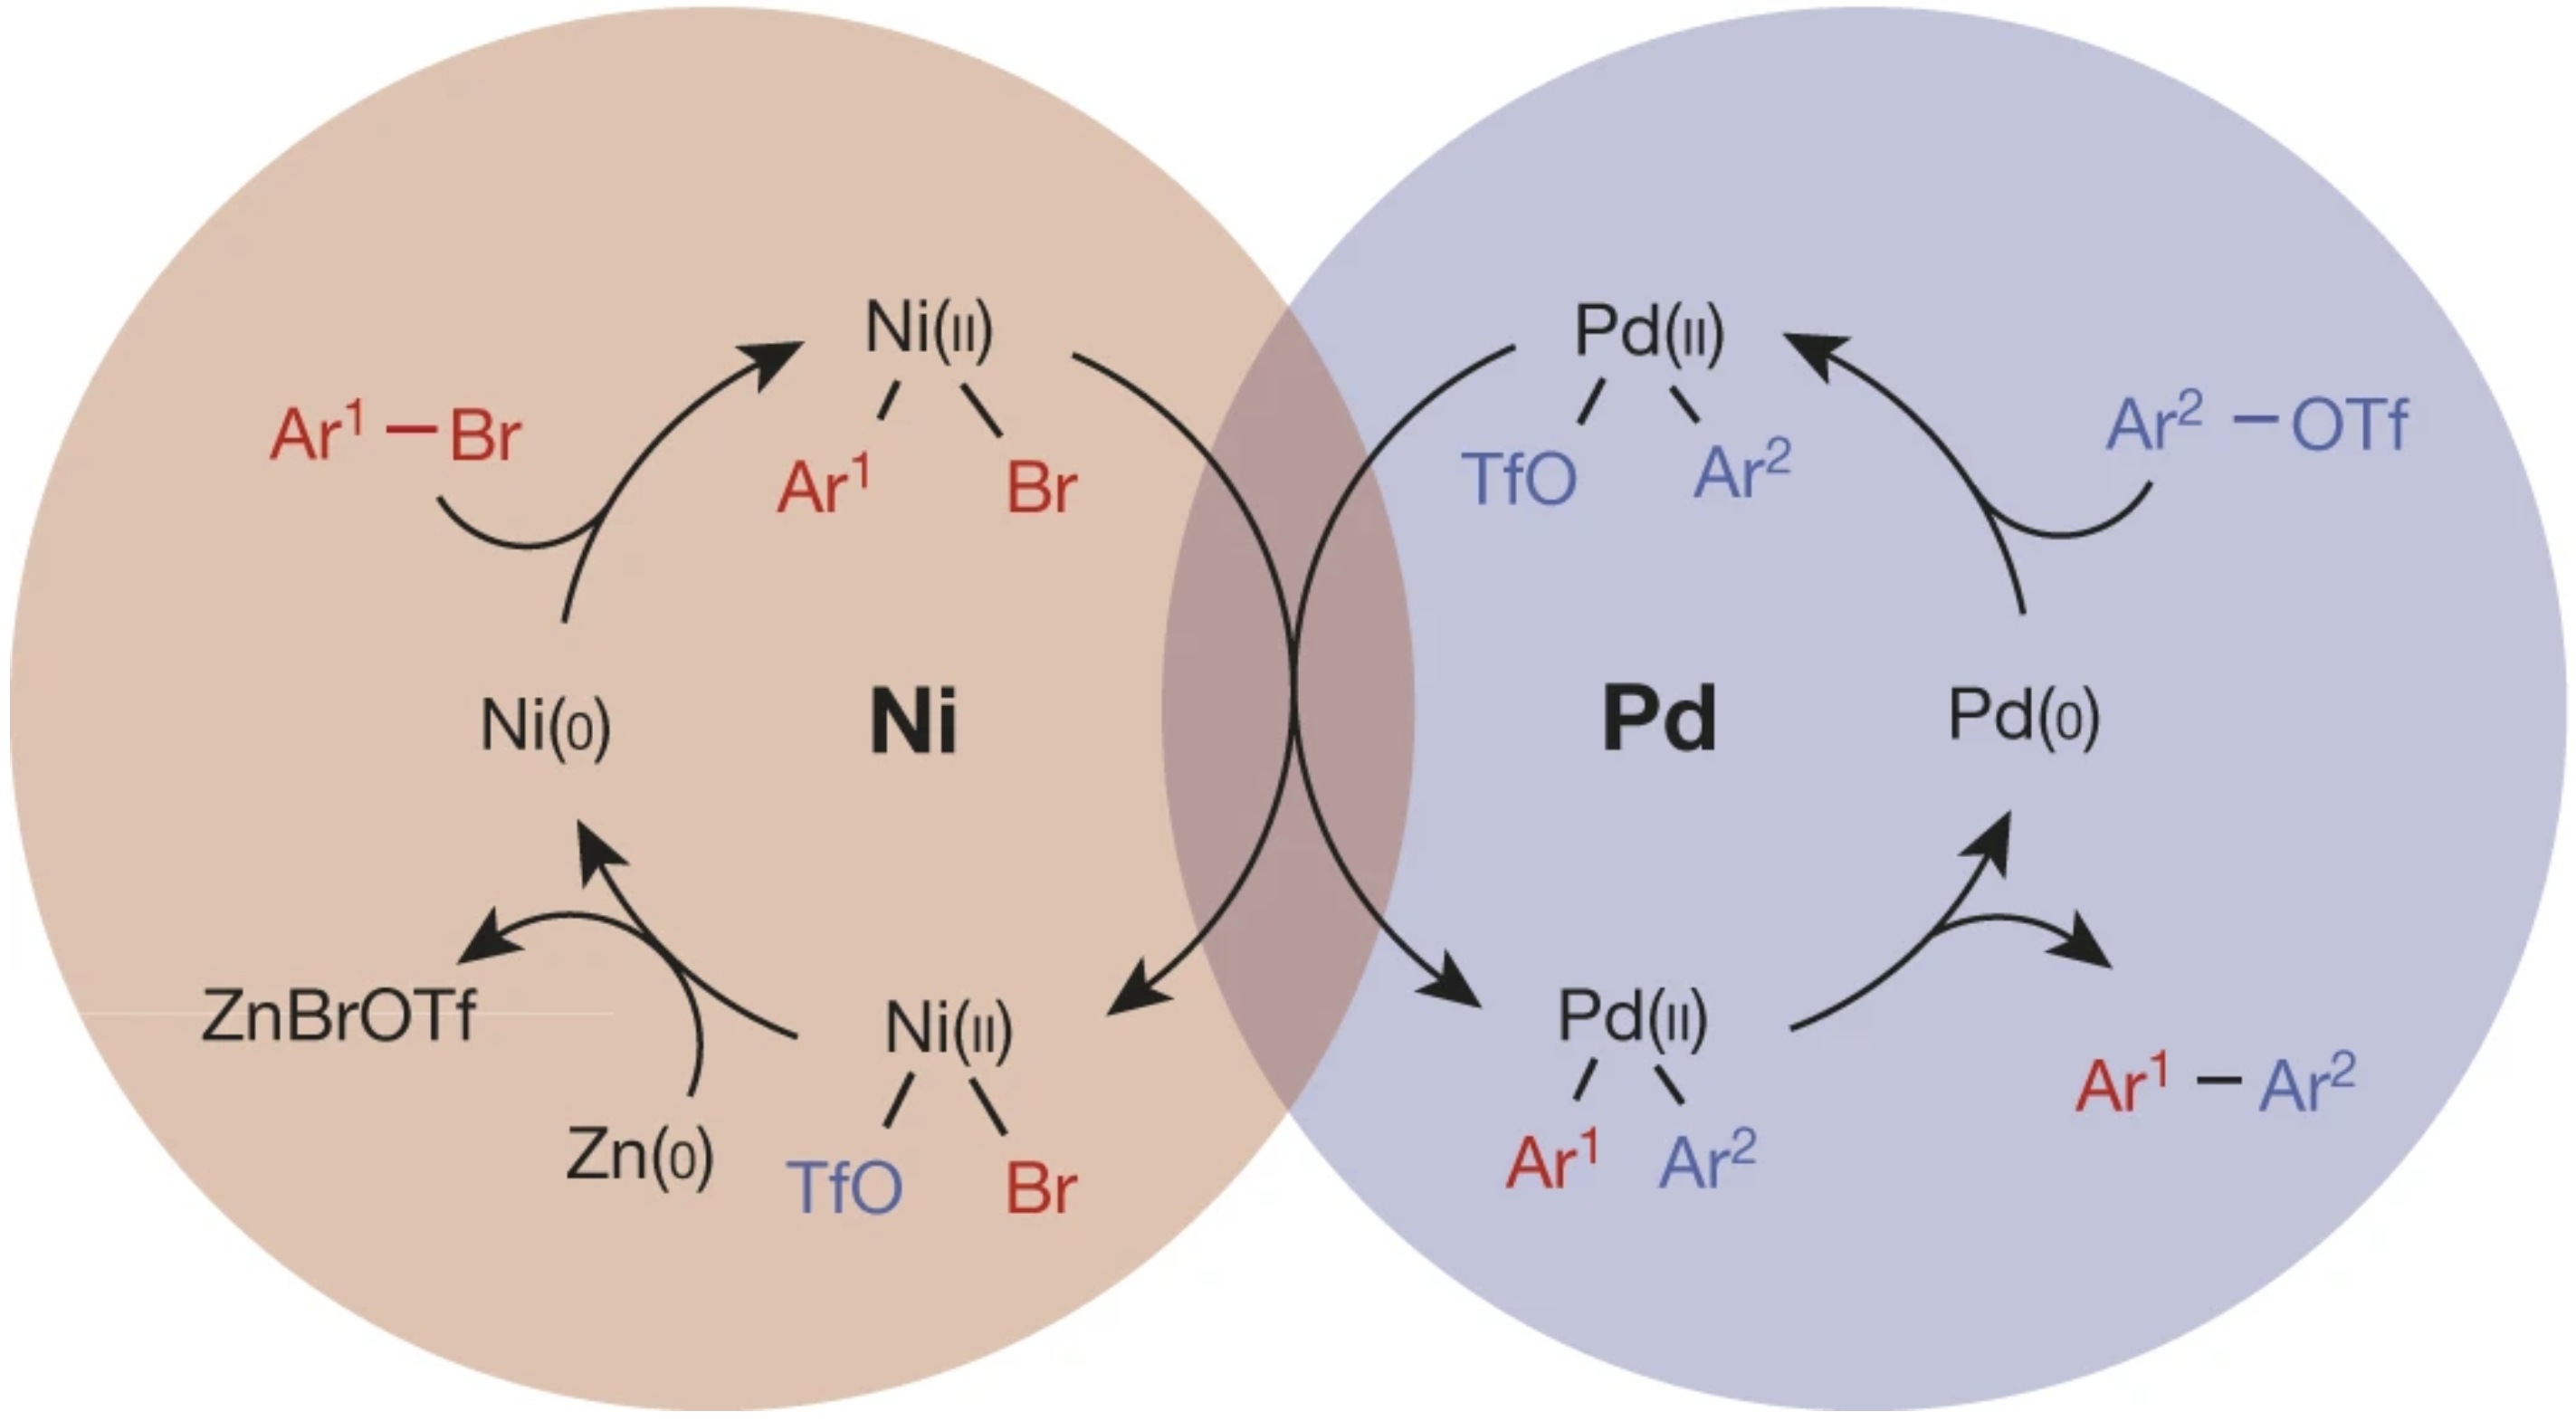
\includegraphics[width=0.6\linewidth]{NiPdCat.png}
        \caption{Tandem nickel-palladium catalyzed aryl halide cross-coupling.}
        \label{fig:NiPdCat}
    \end{figure}
    \begin{itemize}
        \item Combination catalysis can achieve direct cross-coupling of two aryl halides.
        \begin{itemize}
            \item This confers major advantages from a process chemistry perspective, as opposed to having to metallate one of them first.
        \end{itemize}
        \item Weix's tandem catalytic system uses nickel/palladium dual catalysis.
        \begin{itemize}
            \item Nickel's ligand is dtbbpy.
            \begin{itemize}
                \item \ce{{}^{\emph{t}}Bu}tylation of bpy gives better solubility!
            \end{itemize}
            \item Palladium's ligand is dppp.
            \begin{itemize}
                \item Because dppp has three carbons, the chelate effect is weakened to the point that one phosphine can pop off (as I suggested to Paul Chirik!).
            \end{itemize}
            \item Mixed-ligand square-planar species??
        \end{itemize}
        \item The advantage of this dual catalysis is that different metals do oxidative addition at different rates, so you can get transmetallation as if you'd used a different metal.
        \begin{itemize}
            \item \ce{Ni} prefers $\ce{C-Br}>\ce{C-Cl}>\ce{C-OTf}$.
            \item \ce{Pd} prefers $\ce{C-OTf}>\ce{C-Br}>\ce{C-Cl}$.
        \end{itemize}
        \item Although limited to a very narrow scope of pyridine derivatives, this is being used very widely!
        \item References.
        \begin{itemize}
            \item \textcite{bib:Weix1} --- original report.
            \item \textcite{bib:Weix2} --- update for heterocycles.
            \item \textcite{bib:Weix3} --- review of cross-elecrophile couplings.
        \end{itemize}
    \end{itemize}
    \item Pyridine synthesis.
    \begin{itemize}
        \item \textbf{Hantzsch pyridine synthesis} is particularly important.
        \item \textbf{Cyclotrimerization} is most aesthetically pleasing, but not necessarily the most useful.
        \item \textbf{Petrenko-Kritschenko} is a variation on a theme.
    \end{itemize}
    \item Dicarbonyl approaches.
    \begin{itemize}
        \item Scope-limiting factor is often how you get to the dicarbonyl.
        \item Oxidation can be done with nitric acid or DDQ (particularly on a small scale).
    \end{itemize}
    \item Asymmetric pyridines.
    \begin{itemize}
        \item Do Hantzsch chemistry in two-steps.
        \item First, make your preferred $\alpha,\beta$-unsaturated ketone.
        \item Then combine it with a \textbf{vinyligous urethane} (not an enamine) and oxidize.
        \item Advantage: The presence of pyridinium eliminates the need to oxidize at the end.
    \end{itemize}
    \item Kr\"{o}hnke.
    \begin{itemize}
        \item Make the $\alpha$-halo species \emph{in situ}, which reacts with pyridine.
        \item Then enolization, addition, and condensation.
    \end{itemize}
    \item $[2+2+2]$ pyridine synthesis.
    \begin{itemize}
        \item Has been used in some contexts in very large scale, though not for pyridine synthesis.
        \item Ramsay (aged 24) discovered this.
        \item Chemistry in the 1800s was chemistry of "gentlemen," who did things in their home laboratories.
        \item Original report: Acetylene (explosive) plus \ce{HCN} (toxic) in a hot tube gives pyridine.
        \item B\"{o}nnemann picks this up.
        \begin{itemize}
            \item Two acetylenes combine with a cobalt catalyst.
            \item Then Diels-Alder onto the nitrile.
        \end{itemize}
        \item Cyclotrimerizations are cyclotetramerizations have the regioisomer problem, though.
        \item Wittig started the use of these to make aromatics.
        \item If you have a regioisomer problem, cheat by either doing intramolecular stuff or a large excess of one reagent (e.g., as Vollhardt did).
    \end{itemize}
    \item Zincke chemistry.
    \begin{itemize}
        \item A chemist's hope in life is that you develop a reaction, somebody uses it to do something useful, and you get some of the credit or benefit of it. Sometimes this happens during your lifetime, and sometimes after.
        \item Zincke's chemistry found utility 90 years after he died in an ingenious synthesis of strychnine \parencite{bib:ZinckeStrychnine}.
    \end{itemize}
    \item Modern Zincke chemistry: \emph{meta}-halogenation of pyridines via reversible ring-opening.
    \begin{figure}[H]
        \centering
        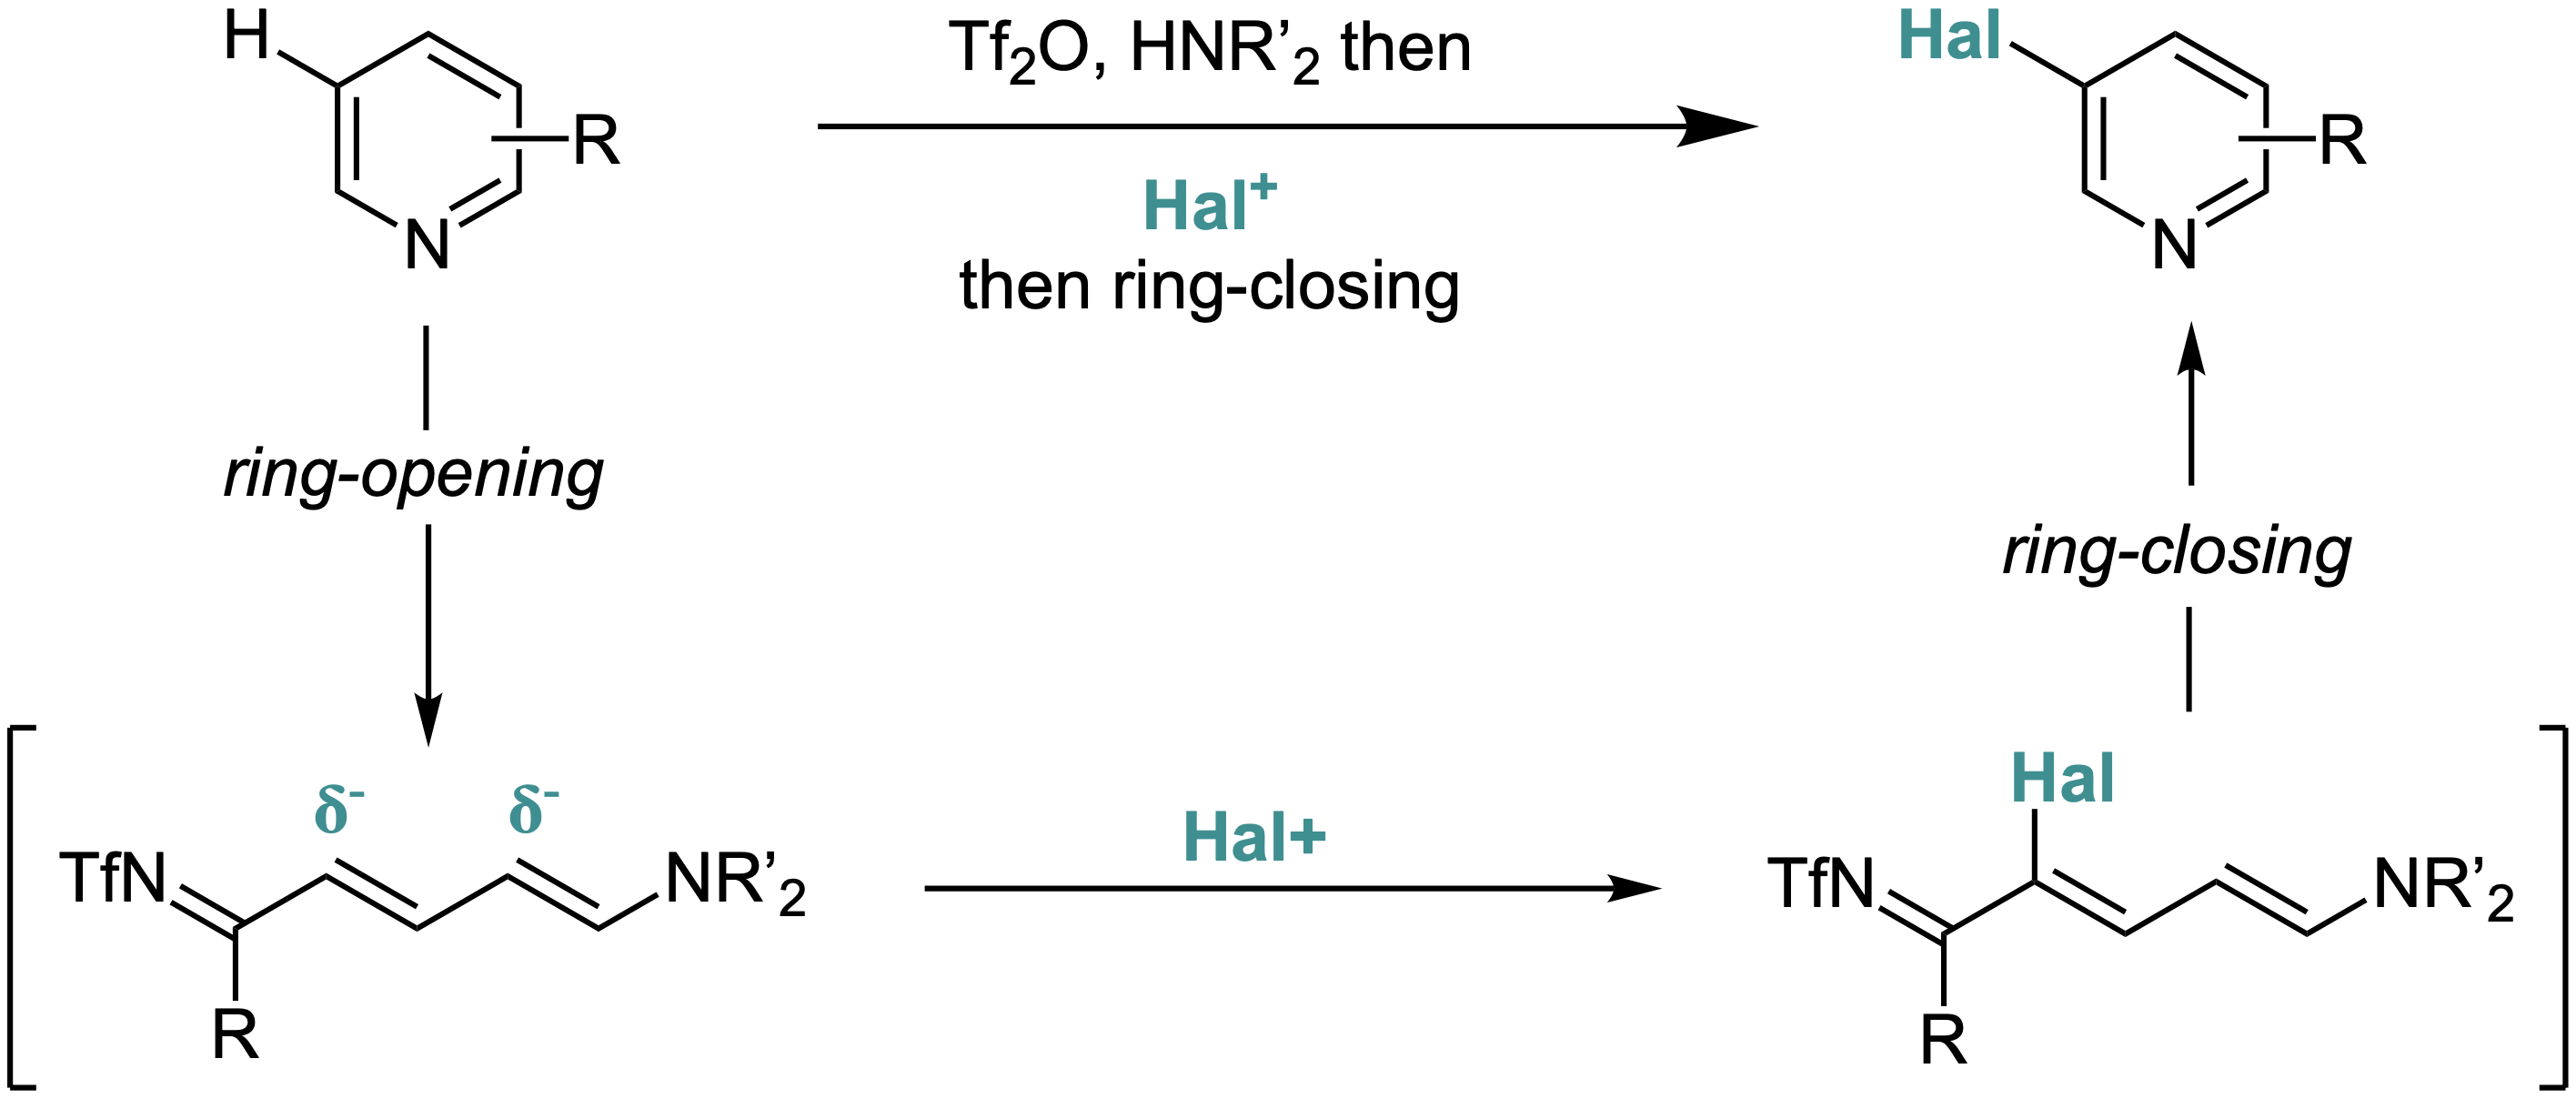
\includegraphics[width=0.6\linewidth]{ZinckeMeta.png}
        \caption{\emph{meta}-halogenation of pyridines via Zinke chemistry.}
        \label{fig:ZinckeMeta}
    \end{figure}
    \begin{itemize}
        \item After Vanderwal's efforts, Zincke chemistry once again lay fallow for a while. But then Andy McNally (Colorado State) used it for \emph{meta}-CH activation.
        \item \ce{Hal+} is some kind of positive halogenating agent.
        \item Mechanism.
        \begin{itemize}
            \item Retrocyclization ring-opens pyridine following triflation.
            \item This temporarily makes pyridines reactive with electrophiles!
        \end{itemize}
        \item Regiochemical ambiguity with NCS; very selective with NBS or NIS.
        \begin{itemize}
            \item They had no clue why, so did DFT and Hammond-type arguments about early/late transition states.
        \end{itemize}
        \item Very elegant paper; eventually came up with good procedures for two types of compounds.
        \item Reference: \textcite{bib:ZinckeMeta}.
        \item Takeaway: Heterocycles are not rocks; balance thinking of them as benzene analogs with thinking of them as normal molecules that can open, close, move around, come from different things, etc.
    \end{itemize}
    \item \emph{meta}-halogenation of pyridines via reversible dearomatization.
    \begin{figure}[h!]
        \centering
        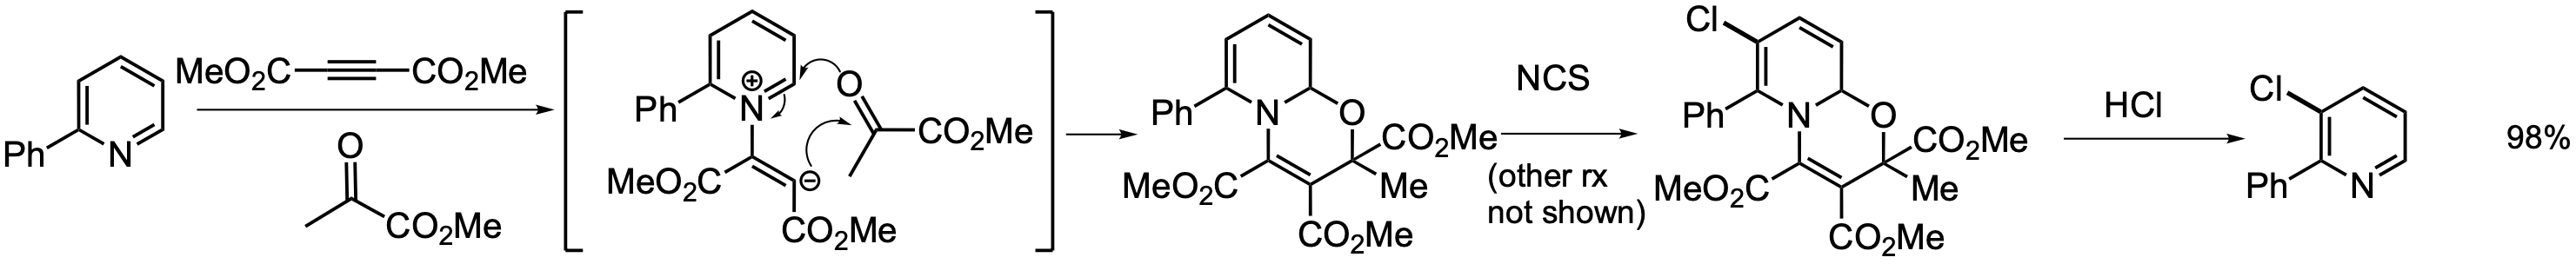
\includegraphics[width=0.99\linewidth]{DearoMeta.png}
        \caption{\emph{meta}-halogenation of pyridines via temporary dearomatization.}
        \label{fig:DearoMeta}
    \end{figure}
    \begin{itemize}
        \item Studer (M\"{u}nster, top German school for OChem) develops this chemistry in the same time frame as McNally.
        \item Again, different products for chlorination vs. bromination.
        \item Take yields like 98\% with a grain of salt, but it indicates that you're probably high-yielding.
        \item Reference: \textcite{bib:DearoMeta}.
    \end{itemize}
    \item Might do some problems on Monday!
    \item Steve covers the synthesis of Nexavar.
    \item Synthesis of a Chk1 Kinase inhibitor.
    \begin{itemize}
        \item Starting material is a bromo/chloro/nitro-substituted 7-azaindole.
        \begin{itemize}
            \item Steve wasn't quite sure how they got here, but his former postdoc is now the head of process chem at Genentech (lmao), so he was able to point Steve toward the route.
        \end{itemize}
        \item Strong acids protonate the pyridine, then add to the 3-position!
        \begin{itemize}
            \item We'll talk more about this later in the course.
        \end{itemize}
        \item Piperidine's amine reacts much faster than the amide.
        \item Amino-indoles are very prone to oxidation, but acylating it immediately gives a clean compound.
        \item Lots of process chem involves what you can do in the same flask; this is \textbf{telescoping}.
        \item But you don't want to do this so much that you have too many impurities to easily filter out.
        \item At scale, you can do some extractions, but you mostly want to do crystallizations.
        \item Different crystalline forms of the same compound can have different patents, different patent lifetimes, different pharmacokinetics, etc.
    \end{itemize}
    \pagebreak
    \item Kinases are responsible for many different physiological functions
    \begin{itemize}
        \item 700 in the body.
        \item Steve thinks it's a miracle we can design molecules to hit 1 out of the 700!
    \end{itemize}
    \item Another kinase synthesis.
    \begin{itemize}
        \item Synthesis is done from commercial pyrazole using Claisen chemistry and then amide formation.
    \end{itemize}
    \item Pharmaceuticals are also widely applied in agrochemistry.
    \begin{itemize}
        \item If you work for Cortiva in Minneapolis, it's gonna be quite similar to Lilly in Indianapolis.
        \begin{itemize}
            \item But when you do scale-up for agrochemicals, cost matters much more!
            \item Though with the environmental push to use smaller quantities agrochemicals, cost is mattering less.
        \end{itemize}
        \item Selectfluor is an \ce{F+} equivalent.
        \begin{itemize}
            \item Very active and expensive.
        \end{itemize}
        \item You often put fluorine into molecules to block the site of oxidation; cytochrome enzymes do \ce{C-H} oxidation as a first step in metabolic excretion, and you can block this with fluorination to slow the pharmacokinetics.
        \begin{itemize}
            \item Very activated system, so probably can use a simple catalyst.
            \item 2-halopyridines are \emph{extremely} activated toward oxidative addition as with S\textsubscript{N}Ar; much worse for 3-halopyridines.
        \end{itemize}
        \item If there's a perfect SM but it's only available from one place, the company will raise the price to whatever they want now that they know their compound is important. Also, what if there's a supply chain interruption?
        \begin{itemize}
            \item Companies like to have 3 sources as a general rule.
        \end{itemize}
        \item As it happens, the SM here is very cheap.
        \begin{itemize}
            \item Most fluoridation reactions use the Halex reaction.
            \item Often \ce{KF} and a ton of heat; the fluoro compounds are more stable, so they come out with thermodynamic equilibration.
        \end{itemize}
        \item Each of these steps can be carried out on a large scale, and the most expensive thing anywhere here is \ce{CsF}.
    \end{itemize}
    \item Vinamidium salts are more stable 1,3-dialdehyde equivalents.
    \begin{itemize}
        \item 1,3-dialdehydes do self-Claisen condensations and all kinds of nasty things.
        \item Developed at Merck, then used on scale there.
        \item Can be used to make tri-substituted pyridines!
        \item 2-methyl group is perfectly setup for lateral deprotonation.
        \item PPA (polyphosphoric acid) is a common strong acid. You isomerize the double bond and then do Friedel-Crafts on the aromatic ring.
        \begin{itemize}
            \item Again, heat is better than a fancy catalyst.
        \end{itemize}
    \end{itemize}
    \item Process vs. medchem.
    \begin{itemize}
        \item Mitsunobu, reduction of nitro (with stoichiometric iron and acetic acid as opposed to Ni, Pd, Pt + \ce{H2}).
        \item Donating groups allow for mild halogenation.
        \item Miyaura borylation.
        \item This is an ugly synthesis; protecting groups are never great, and \ce{Pd} at the end increases the chance of contamination.
        \item Made better at process scale! Still has final \ce{Pd} issue, though.
    \end{itemize}
    \item Very non-activated \ce{NH} requires \ce{Pd} catalysis.
    \begin{itemize}
        \item Xantphos, developed at Dutch Shell for hydroformylation but repurposed for \ce{C-N} bond formation.
    \end{itemize}
    \item Key synthetic transformations using pyridine.
    \begin{itemize}
        \item S\textsubscript{N}Ar with heteroatom nucleophiles (\ce{O}, \ce{N}, \ce{S}), or with malonate anions.
        \item \ce{PPh3} can remove an \emph{N}-oxide because of strong \ce{P=O} bond formation!
        \item Alternative to \ce{R$''$MgX}: Zincke chemistry!
    \end{itemize}
\end{itemize}




\end{document}